\begin{comment}
-------------------------------------------------------
A Fejlesztői dokumentáció tartalmazza
- a probléma részletes specifikációját,
- a felhasznált módszerek részletes leírását, a használt fogalmak definícióját,
- a program logikai és fizikai szerkezetének leírását (adatszerkezetek, adatbázisok,
modulfelbontás),
- a tesztelési tervet és a tesztelés eredményeit.
-------------------------------------------------------
\end{comment}

%% ----------------------------------------------{Megoldási terv}
\section{Megoldási terv}
A program működése 2 részre bontható: weboldalra(kliens) és a szerverre.
A weboldalon össze állított adatokat küldjük fel a szerverre, a szerver a megkapott adatok alapján számol. \newline
\subsection{Weboldal}
	A kliens megvalósításához az alábbi technológiák merültek fel : C++/Qt, C\#, JS/HTML. Végül JavaScript-ben lett megvalósítva, első sorban a grafikon kirajzoló (Flot) miatt, de a szerver kommunikáció egyszerűsége is döntő ok volt amellett, hogy egy weboldal bármely gépen egyszerűen megnyitható, kezelhető.\newline
	Egy oldalból áll melyen a felhasználó szerkesztheti az adatokat. Azért nem lettek a részek külön oldalakon megvalósítva, mert az egyik oldalról az adatok átvitele egy másik oldalra nem annyira egyszerű, viszont nincs is olyan komplex az oldal, hogy szükséges legyen több aloldalra szétbontani. 
	Az oldal megjelenés felépítése megtekinthető \ref{fig:weblap_vazlat}-es képen.
	\begin{figure}[h]
	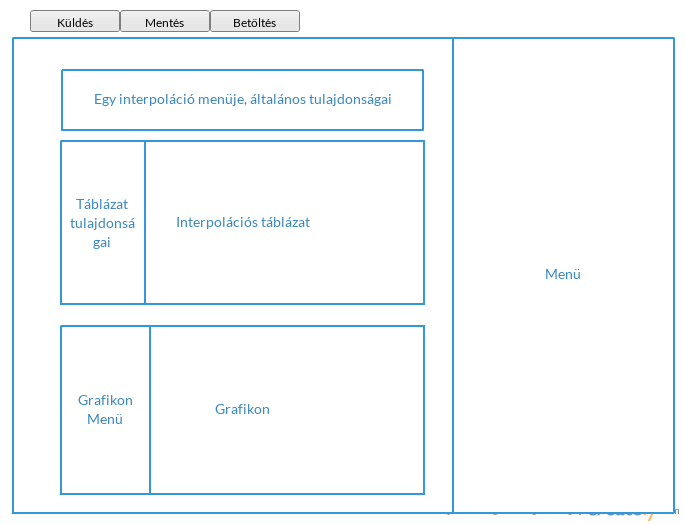
\includegraphics[width=14cm]{pics/weblap_vazlat}
	\centering
	\caption{Weboldal vázlata\label{fig:weblap_vazlat}}
	\end{figure}
	Az első döntés, melyet a felülettel kapcsolatban meg kellett hozni a kirajzolás módja. Mivel JavaScript-hez találtam egy gyorsan megtanulható és kényelmes grafikon kirajzolót, ezért végül webes kliens mellett döntöttem. A grafikon kirajzolóról a \ref{subsec:flot} pontban lehet olvasni.
	A weboldalon meg kell valósítani a pontok dinamikus kirajzolását, és a táblázatos formában történő megjelenítést és szerkeszthetőséget. Mivel több interpolációt küldünk fel a szervernek ezért a weboldalon több szerkesztésére is lehetőséget kell adni. \newline 
	Több interpoláció számítás szerkesztésének megvalósításához kell egy menü rendszer, amelyben eltárolódnak az adatok, és képesek betöltődni.\newline
	Az oldalon input-okat használunk még, és a dinamikus táblázat is JavaScript-ből van legenerálva. A táblázatokban sorok beszúrására teljes táblázat törlésre is lehetőséget kell adni. 
	A táblázatokban inputok vannak az egyes cellákban melyben egyszerű értékek, vagy akár komplexebb objektumok is találhatóak. A bonyolultabb objektumokat json string-ben tároljuk ezekben az inputokban. \newline
	Az interpolációk listájában új adathalmazokat hozhat létre, a régieket szerkesztheti.
	Amikor a felhasználó pontokat, megjelenítést frissít a legtöbb esetben az oldal már a háttérben menti az adatokat a listába. Amikor egy másik interpolációt választunk ki, akkor az betöltődik a táblázatba, és a grafikonba. A módosítások és mentés esetén az aktuálisan kiválasztott interpolációs adathalmaz sora fog frissülni.
	Ha a felhasználó végzett egy gombra nyomással a program legenerálja a szükséges objektumot. \newline
	A felület sok gombot tartalmaz, melyek hatására frissíthetőek az adatok. Amikor frissítünk egy részt, általában mentődnek az értékek egy inputba JSON formában.

\subsection{Elosztott rendszer}
	Az elosztott rendszer megvalósításához az alábbi technológiák merültek fel: \newline C++/PVM, Erlang.
	Miután a JavaScript mellett döntöttem a grafikus felületen, ezután optimálisabbnak tűnt egy hasonlóan gyengén típusos nyelvnek a használata. Az Erlang elég jól támogatja párhuzamosítást és a szerver kommunikációt is, és bár az algoritmusok implementálása nehézkesebb lett volna, de C++-ban megvalósított függvények beépítése miatt ez a probléma megoldódott.
	\newline
	A JavaScript-ből kapott json kibontására talált mochijson segítségével az adatokat át lehetett dolgozni Erlang-os típusokká, alkalmazásáról a \ref{subsec:mochijson} pontban lesz szó.

\subsection{Számítás}
	A számítás megvalósításánál felmerült hogy Erlang-ban legyen, de mivel a számítást ciklusokkal érdemes megvalósítani, ezért egyszerűbb volt egy nem funkcionális nyelvben implementálni azokat.
	A C++-os függvényeket fel lehetett használni az Erlang modulokban. Erre a NIF könyvtárat használtam, melyről az \ref{subsec:nif} pontban részletesen szó esik. 
\subsection{Kommunikáció}
	Amikor a szervert létrehozzuk akkor inicializálunk két processzt. Az egyik a kliens felől várakozik kérésre, a másik a node-ok felől. Amikor egy node fel kíván csatlakozni, küld egy kérést. Ha sikeres volt akkor a szerver ezt jelzi neki, és felkerül a listára. \newline
	A weboldalon egy gomb hatására megy egy kérés a szerver felé. A szerver jó esetben fogadja a kérést. Ha a kliensnek nem sikerült kapcsolatba lépnie a szerverrel, akkor jelzi a felhasználónak hogy a kapcsolódás során hiba lépett fel. \newline
	Ha fogadta a kérést, akkor megpróbálja feldolgozni az adatokat. Ha sikeresen feldolgozta az adatokat, abban az esetben elindul a szétosztás. \newline
	A szétosztás során a felcsatlakozott gépeken létre jönnek a processzek, majd kapnak egy adathalmazt mellyel számolniuk kell. Ha végeztek, az eredményt visszaküldik a szülő processznek. A szülő processz, ha megkapott minden értéket, azt visszaküldi a weboldalnak.
	\newline
	A weboldal sikeres válasz után betölti az eredményeket. 
	\begin{figure}[h]
		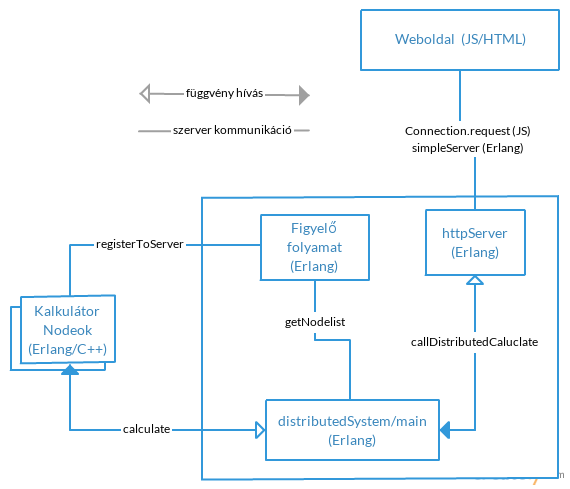
\includegraphics[width=13cm]{pics/kommunikacio1}
	\centering
	\caption{Kommunikáció\label{fig:kommunikacio1}}
	\end{figure}

\section{Felhasznált források és alkalmazásuk}
\subsection{Grafikon kirajzoló - Flot}

	\begin{figure}[h]
	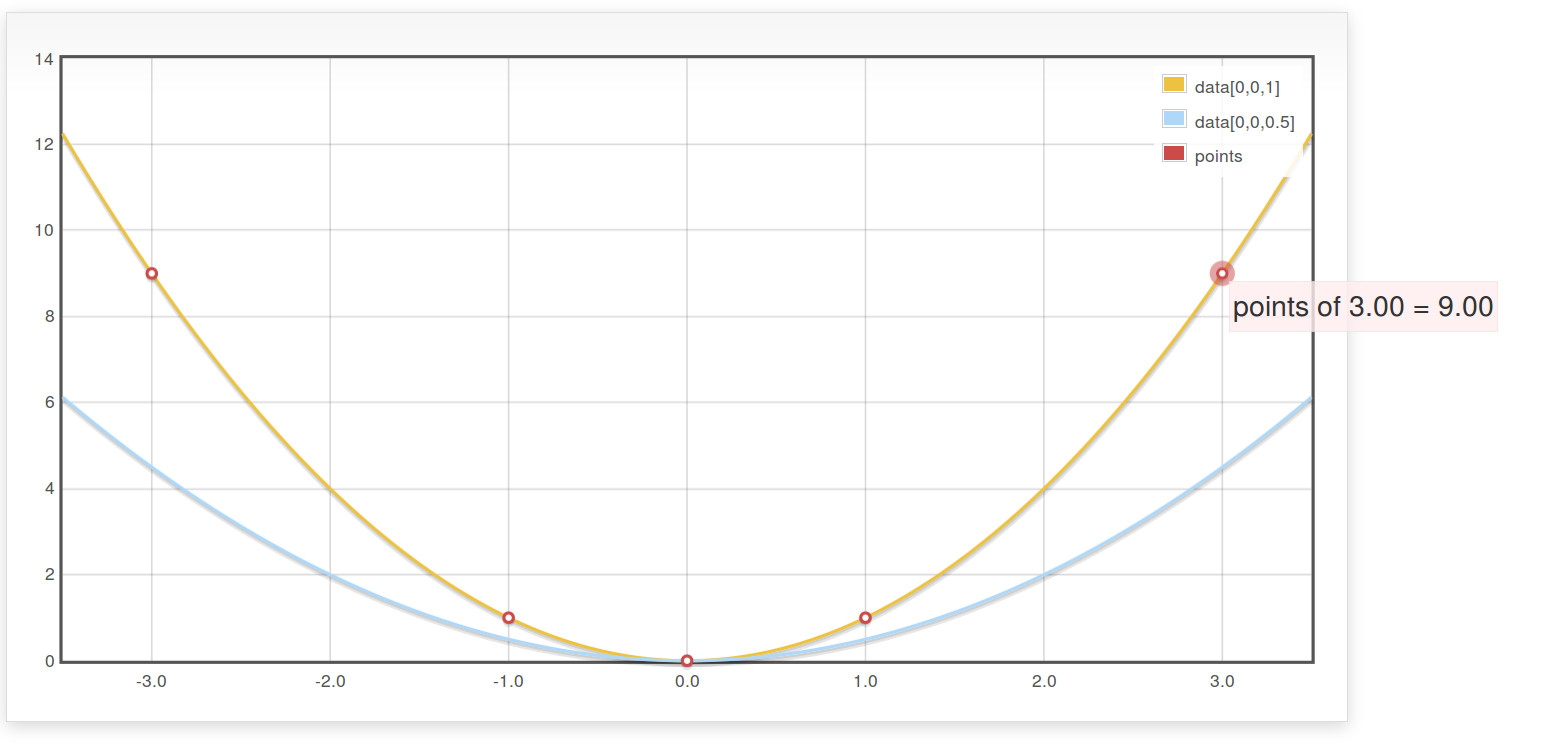
\includegraphics[width=13cm]{pics/plot}
	\centering
	\caption{Grafikon kirajzoló\label{fig:plot}}
	\end{figure}
	
	A Grafikon megjelenítéséhez a Flot-ot használom. Ez egy jQuery-s könyvtár, melyben egyszerűen és látványosan lehet grafikonokat kirajzolni. A forrás a "WebPage/source/flot-8.0.2" mappában érhető el.
	\subsubsection{Felhasználás}
	HTML fájlban egy egyszerű "DIV"-ként jelenik meg, melyet aztán a JavaScript tölt meg tartalommal.
	\begin{verbatim}
	<div id=\"resultplot\" class=\"demo-placeholder\"></div>
	\end{verbatim}
	A JavaScript-ben hivatkozhatunk erre a "DIV"-re, majd az adatok és a típusok segítségével alábbi módon hivatkozhatjuk meg: 
	\begin{verbatim}
	var placeholder = $("#resultplot");
	var plot = $.plot(placeholder, flot_data, type);
	\end{verbatim}
	A paraméterezése a grafikon kirajzolónak az alábbi: 
	\begin{description}
		\item[placeholder] \hfill \\ 
 			DIV hivatkozása
 		 \item[type] \hfill \\ 
 			Megjelenítendő grafikon típusa
 			\newline
 			A Flot sok lehetőséget nyújt a típusok kiválasztására, és ezekre való példákból megalkottam a saját típusomat mely a következőket tartalmazza egy objektumban:
	 		\begin{verbatim}
				series: { line: { show: true } } 
	 		\end{verbatim}
			Beállítjuk hogy a vonalakat jelenítse meg. Ekkor a pontokat is megjeleníti, a többi beállítás függvényében.
	 		
	 		\begin{verbatim}
				xaxis: { zoomRange: [0.1, 1], panRange: [-1000, 1000] }
				yaxis: { zoomRange: [0.1, 100], panRange: [-1000, 1000] }
	 		\end{verbatim} 
	 		X és Y koordinátákon nagyítás és mozgatási beállítások interaktívvá állítása
		 	\begin{verbatim}
				grid: { hoverable: true, clickable: true }
		 	\end{verbatim} 
		 	Ezeket a tulajdonságokat használjuk arra hogy felvegyünk új pontokat.\newline
		 	Emellett ha ráviszem az egeret az egyik pontra, megmutatja a pont koordinátáját, és értékeit, és hogy melyik ponthalmazon van.
		 	\begin{verbatim}
				zoom: { interactive: true}, pan: { interactive: true }
		 	\end{verbatim} 
		 	Nagyítás és kattintással mozgatás engedélyezése. \newline
			Ennek a beépítésével is foglalkoztam, de a kattintás sajnos nem egyeztethető könnyen össze a pont figyeléssel, valamint a beépítés után lassú lett, és akadozott a felület, így végül az interaktivitását külső komponensekkel(inputokkal) oldottam meg.

 		\item[flot\_data] \hfill \\ 
 		A tényleges adathalmazokat tartalmazó tömb, melyben az egyes adatokról egyéni információkat is tartalmazza.\newline
 		\begin{description}
			\item[data] \hfill \\ 
			Pontok halmaza, melyeket megjelenítünk\newline
			[x, y] pontokból álló tömb\newline
			Polinom esetén is ezt használjuk, ezért a polinom behelyettesített értékeit adjuk itt meg. Amikor az egérrel felé megyünk ezeket a pontokat fogja megjeleníteni.
			\item[label] \hfill \\ 
			Adathalmaz elnevezése, ezt láthatjuk amikor az egérrel a pont felé visszük az egeret, valamint a színek-elnevezések össze párosításánál is segít.
			\item[points] \hfill \\ 
			Ha pontokat kívánunk megjeleníteni, akkor ezt a kapcsolót kell alkalmazni.
			\item[lines] \hfill \\ 
			Ha a pontokból alkotott vonalat kívánunk látni, akkor ezt a kapcsolót kell alkalmazni. Ezt használjuk a polinom megjelenítéséhez.
		\end{description}
 		\begin{verbatim}
		var example_datas = [{
		    data: d4,
		    label: "neved4",
		    lines: { show: true }
		}, {
		    data: d3,
		    label: "neved43"
		    points: { show: true }
		}];
		\end{verbatim}
	\end{description}

\subsection{Http szerver}
	A szerver kommunikációt Erlang oldalon 2 megtalált minta fájlból állítottam elő. Az egyikben egy egyszerű szerver kommunikációt mutattak be Erlang-ban\cite{simpleserver}. \newline
	A másik pedig az Erlang dokumentációjában megtalálható minta kommunikáció tcp protokollal\cite{tcpserver}.

\subsection{Ping-pong Node figyelő}
	http://www.erlang.org/doc/getting\_started/conc\_prog.html
	Az Erlang oldalán található dokumentációban, mely az elosztás és a node kommunikációt mutatja be, sok minta kódot tartalmaz, melyekből könnyen elő tudtam állítani a saját kódomat.\newline
	Ez alapján a párhuzamosítottan számoló programomat könnyen át tudtam alakítani elosztott módon számítóvá. \newline 
	Emelett kellett valami lehetőség arra hogy a gépek fel tudjanak csatlakozni a szerverre. Lehetőség lett volna arra is hogy a figyelő helyett csak megkapja a gépek listáját a szerver, de így tisztábban szét van választva a háttér és a kliens, és nem is szükségesek a tényleges számításhoz. \newline
	Ezen az oldalon található minták a ping-pong kommunikációra, melynek segítségével hoztam létre a node-figyelőt. Ez a modul a \texttt{ServerConfig/nodeWatcher.erl} fájlban található meg. \newline

	Ennek mintájára hoztam létre az alábbi figyelőt, melyet regisztrálunk \texttt{pid\_watcher} atom segítségével. 
	\begin{verbatim}
	startPidWatch() ->
	    PidWatch = spawn(nodeWatcher, pidWatch, [self(), []]),
	    register(pid_watcher, PidWatch),
	    PidWatch.
	\end{verbatim}

	A másik gépről ezután lehet küldeni egy "ping"-et, melyet megkap a node-figyelő.
	\begin{verbatim}
	registerToServer(Pong_Node) ->
	    spawn(nodeWatcher, registerToServerNode, [Pong_Node]).
	...
	registerToServerNode(Pong_Node) -> 
	    {pid_watcher, Pong_Node} ! {worker_write, self(), node()},
	    ...
	\end{verbatim}


\subsection{Struktúra kezelő: mochijson}
	A mochijson egy Erlang-hoz is használt modul, melynek segítségével egy json string-et át lehet konvertálni Erlang-os struktúrává. \newline 
	\texttt{git clone https://github.com/mochi/mochiweb.git}(2015.05)
	paranccsal a teljes mochiweb könyvtárat le lehet tölteni. A \texttt{mochiweb/src} mappában találhatóak azok a fájlok melyeket le lehet fordítani, és be lehet tölteni az Erlang shell-be. Lehet letölteni a fájlokat különállóan is. \newline
	Eredetileg csak a mochijson.erl-re volt szükségem, de miután komplexebb adatot kellett encode-olnom szükségessé vált még egy fájl betöltése, viszont nem tudtam hogy az még milyen függőségeket hordoz magában, így letöltöttem az egész repository-t. \newline
	Ha Erlang-ban lefordítjuk shell-ben \texttt{mochijson:encode, decode} függvényekkel egyszerűen lehet használni.\newline 
	Példa képen megtekinthetjük az alábbi egyszerű json-t, mely már tartalmaz objektumot és tömböt.
	\begin{verbatim}
		{
		    "1": {
		        "result": [
		            0.1,
		            0.5,
		            0.7
		        ],
		        "time": 0.5
		    }
		}
	\end{verbatim}
	Ennek string formájára meghívhatjuk a mochijson decode függvényt.
	\begin{verbatim}
	ErlStruct = mochijson:decode(
	    "{\"1\":{\"result\":[0.1,0.5,0.7],\"time\":0.5}}"
	).
	\end{verbatim}
	Ennek eredménye egy Erlang-os struktúra.
	\begin{verbatim}
		{struct, [
		    {"1", {struct,[
		          {"result",{array,[0.1,0.5,0.7]}},
		          {"time",0.5}
		    ]}}
		]}
	\end{verbatim}
	Az \texttt{mochijson:encode} segítségével pedig ezt a struktúrát vissza tujduk alakítani json string-gé. Bár az eredményt shell-ben binary formában lehet egyszerűen megtekinteni, és ebben a formában is kell vissza küldeni a kliensnek. 
	\begin{verbatim}
		iolist_to_binary(mochijson:encode(ErlStruct)).
		<<"{\"1\":{\"result\":[0.1,0.5,0.7],\"time\":0.5}}">>
	\end{verbatim}


	\subsubsection{Felhasználás}
	Ennek a típusa nem egyszerű, főleg ilyen komplex adathalmaznál. Ennek kezelésére létre lett hozva a Utility/structHandler modul. \newline 
	Első lépésben a string-et konvertáljuk a kellő típussá. 
	\begin{verbatim}
		getDataByJson(JsonSting) -> apply(mochijson, decode, [JsonSting]).
	\end{verbatim}
	Ismeretek segítségével létre hoztam egy olyan függvényt, ami kinyer egy adott értéket a struktúrából.
	\begin{verbatim}
		getElementByKey(array, {array, Array}) -> Array;
		getElementByKey(struct, {struct, Array}) -> Array;
		getElementByKey(Name, {struct, Struct}) -> getElementByKey(Name, Struct);
		getElementByKey(Name,[{Name, Value}]) -> Value;
	\end{verbatim}
	Ennek felhasználásával dolgoztam fel a struktúrát.

\subsection{Erlang modul C++-ban : NIF}
	NIF \cite{erl_nif} (native implemented functions) egy C könyvtár, melynek segítségével implementálhatjuk egy modul függvényeit C-ben vagy C++-ban. 
	\subsubsection{Felhasználás}
	A calculator Erlang-modul megvalósítását C++-ban implementáltuk.\newline
	Calculator/ mappában található erlang.cpp és a calculator.erl fájlokban használjuk fel a NIF-et.
	Amely fájlban végezzük a modul közvetlen kommunikációját az Erlang-al ott le kell tölteni az \texttt{erl\_nif} könyvtárat.
	\begin{verbatim}
		#include "erl_nif.h"
	\end{verbatim}
	Emellett meg kell neki adni, melyik függvényeket, hány paraméterrel szeretnénk az Erlang-ba betölteni. 
	A fájlt \texttt{Calculator/erlang.cpp} néven találhatjuk meg.
	\begin{verbatim}
		static ErlNifFunc nif_funcs[] = {
		    {"calculate", 4, calculate_nif}
		};
	\end{verbatim}
	Amikor inicializáljuk, le kell írni hogy melyik modul-nak lesz a része. 
	\begin{verbatim}
		ERL_NIF_INIT(calculator, nif_funcs, NULL, NULL, NULL, NULL)
	\end{verbatim}
	Amikor meghívódik az Erlang-ból ez a modul, paraméterként \texttt{ERL\_NIF\_TERM} típusú változókat kapunk, melyeket lehetőség van átkonvertálni C++-os típusokká. \newline
	Az \texttt{enif\_get\_int} függvény segítségével egy változóból kinyerhetjük az integer-ré konvertált értékét. Hasonlóan használjuk az \texttt{enif\_get\_double} függvényt mely értelem szerűen egy double típusú értéket ad vissza.
	\newline
	Egy lista elemeit \texttt{enif\_get\_list\_cell} függvény segítségével tudtam átkonvertálni. 
	Ennek segítségével megvalósítottam a vektor-rá és mátrix-á alakító függvényeket,
	\begin{verbatim}
		ERL_NIF_TERM head; ERL_NIF_TERM tail = arg;
		//...
		while(enif_get_list_cell(env, tail, &head, &tail)) {
		    //...
		}
	\end{verbatim}
	A számítás eredménye egy vektor, így az eredményül kapott értéket vissza kell valahogyan konvertálni Erlang-os típussá. Ezt az \texttt{enif\_make\_double} és az \texttt{enif\_make\_list\_from\_array} függvények segítségével lehet megvalósítani. 
	Ennek implementálása a \texttt{convertList} függvényben történt.
	\newline
	A tényleges híváshoz a \texttt{nif\_funcs}-ban meghivatkozott \texttt{calculate\_nif}-et kell implementálni. \newline
	Ebben meghívódnak a kovertáló függvények a helyes paraméterezés kialakításához, majd az eredménnyel vissza térünk egy lista formájában.
	\begin{verbatim}
	static ERL_NIF_TERM calculate_nif(ErlNifEnv* env, int argc, const ERL_NIF_TERM argv[]) {
	    //...
	    poli = interpolateMain(X, Y, type, isInverse);
	    return convertList(env, poli);
	}
	\end{verbatim}

\subsection{Dokumentációhoz felhasznált programok}
	A tervezési, és megvalósítási szemléltető képek és diagramok egy webes szerkesztő segítségével valósultak meg. Ez az oldal 2015-ben a http://creately.com/ címen volt elérhető.

\section{Megvalósított mappaszerkezet}

A fájlszerkezetnek a tervezésénél nem voltak a belső részek komolyabban megtervezve, dinamikusan változtak. 3 mappa volt a tervezett: elosztott rendszer, weboldal és a külső fájlok mappája. A többi mappa mind a külsők, és a belsők a fejlesztés során lettek bele tervezve, amikor a fájlok mennyisége, vagy az új technológia szeparálása megkívánta azt.

\begin{figure}[h]
	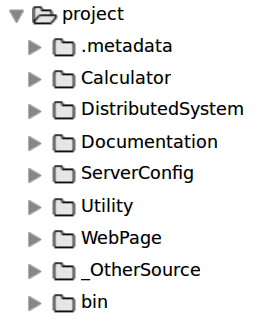
\includegraphics[width=5cm]{pics/folders_all}
	\centering
	\caption{Külső mappaszerkezet\label{fig:folders_all}}
\end{figure}

\begin{description}
	\item[Calculator] \hfill \\ 
		Az interpoláció számítás megvalósítását valamint az Erlang-modullá alakítását is tartalmazó mappa.
		Függvényei a DistributedSystem mappából hívódnak.
	\item[DistributedSystem] \hfill \\ 
		Elosztás logikáját tartamazó mappa, melynek függvényei a ServerConfig mappából hívódnak. 
	\item[ServerConfig] \hfill \\ 
		Szerver megvalósítását tartalmazó mappa.
	\item[Utility] \hfill \\ 
		Több helyen is meghívható függvényeket tartalmazó mappa.
		Struktúra kezelés megvalósítása és a mochijson található itt. 
	\item[WebPage] \hfill \\ 
		Weboldal mappája. 
	\item[\_OtherSource] \hfill \\ 
		Külső felhasznált komponensek mappája.
	\item[bin] \hfill \\ 
		Szerver inicializálását tartalmazó mappa. Ide kerülnek a lefordított fájlok is.
	\item[Documentation] \hfill \\
		Dokumentáció forrás fájljait tartalmazó mappa. 
\end{description}

%% ----------------------------------------------{Weboldal}
\section{Weboldal megvalósítása}
\subsection{Felépítés}
	A weboldal forráskódja a /webpage mappában helyezkedik el. 
	A fájlszerkezet az alábbi:
	\begin{figure}[h]
		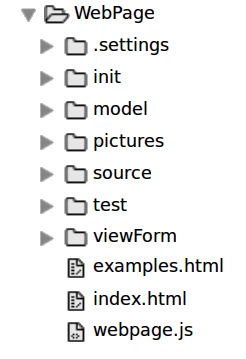
\includegraphics[width=4cm]{pics/folders_webpage}
		\centering
		\caption{A weboldal mappái\label{fig:folders_all}}
	\end{figure}
	\begin{description}
		\item[webpage.js :] \hfill \\  
		Globális változók inicializálása és pár alapbeállítás lefuttatása
		
		\item[webpage.html :]  \hfill \\ 
		Weboldal megjelenítése, fájlok betöltése
		
		\item[/init] \hfill \\ 
		Inicializáló függvények hívásai és események
		\begin{description}
			\item[menulist.js : ] \hfill \\ 
				Interpolációk listájának inicializálója
		  	\item[plot.js : ] \hfill \\ 
		  		Interpolációs grafikon inicializálása
			\item[table.js : ] \hfill \\ 
				Interpolációs táblázat inicializálása
		 	\item[events.js : ] \hfill \\ 
		 		Gombra kattintások eseményei
		\end{description}

		\item[/model] \hfill \\ 
		Objektumok, melyeket az inicializáló lépésben hívunk, és azok segédletei
		\begin{description}
		 	\item[base.js : ] \hfill \\
		 		Globális függvények \newline
		 		Base.get, Base.erlangJSON, Base.forEach
		 	\item[base\_table.js : ] \hfill \\
		 		Általános táblázat generáló függvény
		 	\item[connection.js : ] \hfill \\
		 		Szerver kapcsolat meghívására szolgáló függvény \newline
		 		Connection.request
		 	\item[plot\_types.js : ] \hfill \\
		 		A grafikon kirajzoló típus objektumai
		 	\item[polinome.js : ] \hfill \\  
		 		Polinom kirajzolását segítő függvények \newline
		 		makePolinome található benne és egyéb segédfüggvények
		 	\item[web\_page\_debug.js : ] \hfill \\ 
		 		A Weboldalon történő kiíratást segítő objektum \newline
		 		Jelenleg sehol nem használjuk már, de a megvalósítás során fontos szerepe volt a hibajavításban
		\end{description}
		\item[/model/interpolation] \hfill \\
			Az oldal 3 fő részegységének függvényei
			\begin{description}
			\item[menulist.js : ] \hfill \\ 
				Interpolációk lista megvalósítása \newline
				function interpolationMenulist (aConfig) Objektum fájlja
		  	\item[plot.js : ] \hfill \\ 
		  		Interpolációs grafikon megvalósítása \newline
				function interpolationPlot(aConfig) Objektum fájlja
			\item[table.js : ] \hfill \\
				Interpolációs táblázat megvalósítása \newline
				function interpolationTable(aConfig) Objektum fájlja
			\end{description}

		\item[/test] \hfill \\ 
			Olyan weboldal részlet fájlok, melyekből kialakult a mostani nagy fájl, és az objektumai, valamint tartalmaz még minta adathalmazokat.

		\item[/viewForm] \hfill \\ 
			Megjelenítéssel kapcsolatos css fájlokat tartalmazó mappa.
	\end{description}

\subsection{Fontosabb objektumok és függvények}
	\hfill
	Az objektumokat legtöbb esetben egy függvény generálja, melyeket a visszatérés után felhasználunk az eseménykezelésekhez.
	%%\ref{fig:webpage_big}
	%%\ref{fig:webpage_plot_class}
	%%\ref{fig:webpage_class_table}
	\begin{figure}[h]
		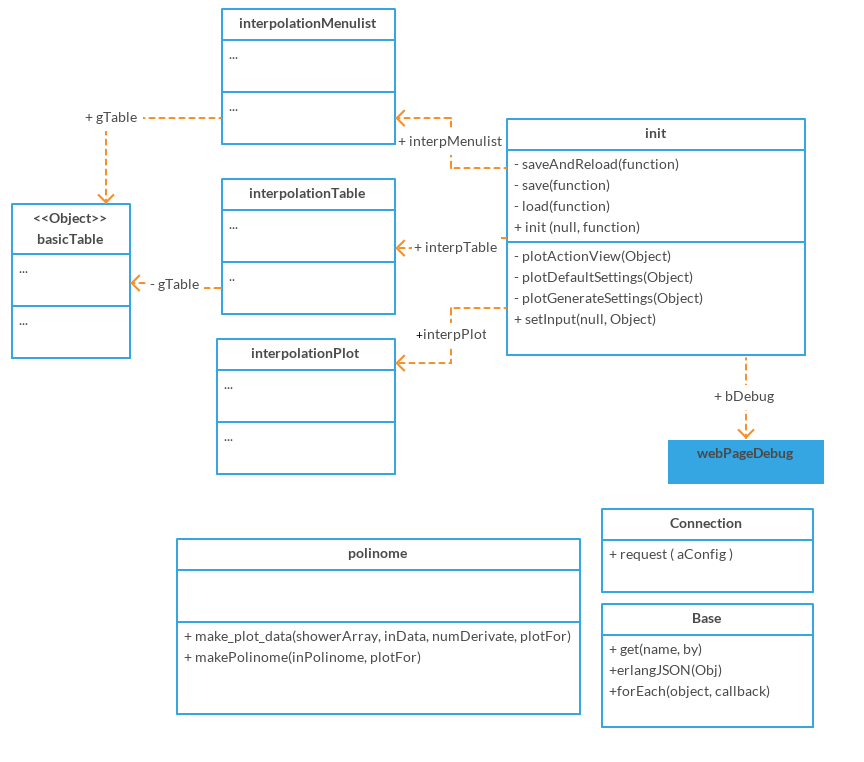
\includegraphics[width=14cm]{pics/webpage_big}
		\centering
		\caption{Weboldal osztálydiagramja\label{fig:webpage_big}}
	\end{figure}

	\begin{figure}[h]
		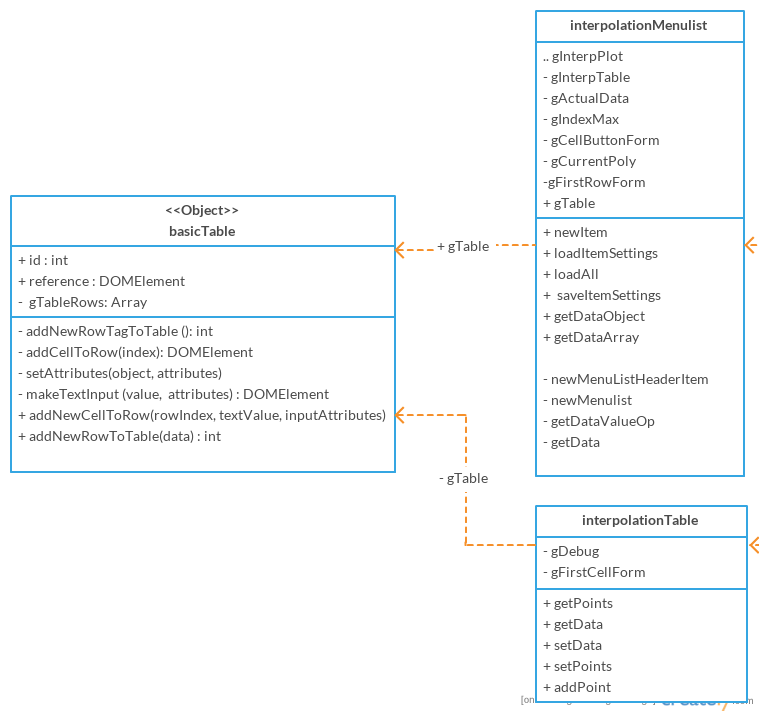
\includegraphics[width=14cm]{pics/webpage_class_table}
		\centering
		\caption{Táblázatok osztálydiagramja\label{fig:webpage_class_table}}
	\end{figure}

	\begin{figure}[h]
		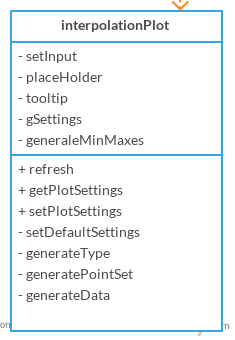
\includegraphics[width=5cm]{pics/webpage_plot_class}
		\centering
		\caption{Grafikon kirajzoló osztálydiagramja\label{fig:webpage_plot_class}}
	\end{figure}

	\begin{description}
		\item[makePolinome(inPolinome, plotFor)] \hfill \\ 
			Polinom pontjainak legenerálására szolgáló függvény, a grafikon kirajzolónak megfelelő típusban
			\begin{description}
				\item[inPolinome] \hfill \\ 
					A polinom tömbös formában.
				\item[plotFor] \hfill \\ 
					A polinom intervalluma és pontossága.
			\end{description}
		\item[Connection.request(aConfig)] \hfill \\ 
			Elküldi a szervernek az értékeket
			\begin{description}
				\item[aConfig.params] \hfill \\
				A kommunikációban a paraméter amelyet átküldünk a szervernek
				\item[aConfig.callback] \hfill \\
				Sikeres visszatérés esetén ez a függvény fut le a szervertől vissza adott válasszal. 
			\end{description}
		\item[basicTable (aConfig)] \hfill \\ 
			Egy alap tábla objektum. Ennek segítségével lehet létrehozni az interpolációs táblázatot és a menü listát(interpoláció választó).
			\begin{description}
			\item[that.addNewCellToRow(rowIndex, textValue, inputAttributes)] 
				\hfill \\  Ad egy új cellát a sorhoz.
			\item[that.addNewRowToTable(data)]
				\hfill \\ Ad egy új sort a táblázathoz.
			\item[that.addNewColumnToTable(data)]
				\hfill \\ Ad egy új oszlopot a táblázathoz.
			\item[that.newTable()] 
				\hfill \\ Új tábla létrehozása.
			\item[that.setCellForm((i , j, attributes))] 
				\hfill \\ Egy adott cella megformázás beállítása.
			\item[that.getNumOfCols()] 
			 	\hfill \\ Visszatér az oszlopok számával.
			\item[that.getNumOfRows()]
				\hfill \\ Visszatér a sorok számával.
			\item[that.getRow(i)]
				\hfill \\ Visszatér a sor DOM-elemével az index alapján.\newline
				Ha nincs olyan indexű akkor null-al tér vissza.
			\item[that.getInputTag(i, j)]
				\hfill \\ Visszatér a tábla input elemével.
			\item[that.getValue(i, j)]
				\hfill \\ Egy adott cella érték lekérdezése.
			\item[that.findValue(column, value)] 
				\hfill \\ Megkeresi melyik sorban van egy adott értéket.
			\item[that.setValue(i, j, value, form)]
				\hfill \\ Beállít egy adott értéket egy cellának.
			\item[that.deleteTable()]
				\hfill \\ Teljesen törli a táblázatot.
			\item[that.remove(row)]
				\hfill \\ Kivesz egy sort a táblázatból.
			\item[addNewRowTagToTable ()]
				\hfill \\ Ad egy új sort a táblázathoz.
			\item[addCellToRow(index)]
				\hfill \\ Ad  egy cellát a sorhoz.
			\item[setAttributes(object, attributes)]
				\hfill \\ Beállítja egy objektum tulajdonságait.
			\item[makeTextInput (value,  attributes)]
				\hfill \\  
				TextInput hozzáadása a sorhoz.
			\end{description}
		\item[interpolationMenulist (aConfig)] 
			\hfill \\ 
			Az interpolációs menü függvénye. Itt tarjuk számon az aktuálisan betöltött adathalmazt.
			\begin{description}
			\item[that.newItem()] 
			\hfill \\ Új elemet vesz fel a listába. Gomb hatására is meghívódhat. \newline Új lista elem egy új interpolációs adathalmaz felvételét jelenti.  
			\item[that.getDataArray(server)] 
			\hfill \\ Visszatér az adathalmazzal, tömb formában. Ebben a formában küldjük fel a szervernek.
			\item[that.getDataObject()] 
			\hfill \\ Eredményül adja az adathalmazt, egy objektum formájában. Az Objektum értékeinek kulcsa, az interpolációk egyedi azonosítója (id-ja).
			\item[that.saveItemSettings()] 
			\hfill \\ Elmenti az adatokat az aktuálisan kijelölt sorba.
			\item[that.loadItemSettings(index)]
			\hfill \\ Feldogozza az adatsort a táblából, és betölti az adatokat a táblába.
			\item[that.loadAll(savedObject, resultObject)] 
			\hfill \\Betölti az összes Interpolációt az adott adathalmazból
			\item[newMenulist()] 
			\hfill \\
			Új menülista: régi menü kitörlése, és egy új generálása
			\hfill \\ 
			\end{description}
		\item[interpolationPlot (aConfig)]
			\hfill \\ Grafikon megjelenítése: "Flot" segítségével létrehoztam az alábbi Objektumot. Ebben valósítottam meg a kirajzolást, és annak tulajdonságait.
			\begin{description}
			\item[that.refresh(points, polynomials)]
			\hfill \\ Pontok és a polinomok alapján frissíti a grafikont.
			\item[that.getPlotSettings]
			\hfill \\ Visszatér a grafikon megjelenítési tulajdonságokkal. Ennek segítségével mentünk.
			\item[that.setPlotSettings]
			\hfill \\ Betölti a grafikon megjelenítési tulajdonságokat.
			\item[generateData(senderData, polynomial)]
			\hfill \\ Legenerálja a grafikon azon bemenő paraméterét, amely a megjelenítendő adatokat állítja.

			\item[generateType()]
			\hfill \\ Legenerálja a grafikon azon bemenő paraméterét, amely a grafikon megjelenítését állítja.
			\item[setDefaultSettings()]
			\hfill \\ Legenerálja a grafikon azon bemenő paraméterét, amely a grafikon megjelenítését állítja.
			\item[generatePointSet(tableArray, derivNum)]
			\hfill \\ Legenerálja az adott pontokat, az interpolációs táblázatból.
			\end{description}

		\item[interpolationTable (aConfig)]
			\hfill \\ 
				Az interpolációs Táblázat logikája, és generálása. Ebben a táblázatban tekinthetjük meg a pontokat.
			\begin{description}
			\item[that.addPoint(x, y, dn)] 
			\hfill \\ Hozzá adja a pontot a táblázathoz. Ha létezik ezen az X-en pont akkor frissíti.
			\item[that.setPoints(tableArray)] 
			\hfill \\ Feltölti a táblázatot egy adott tömb értékeivel.
			\item[that.setData(data)] 
			\hfill \\ Feltölti az adatokkal a táblát.
			\item[that.getData()] 
			\hfill \\ Visszatér a táblázatban szereplő adatokkal.
			\item[that.getPoints()] 
			\hfill \\ Visszatér a táblázatban szereplő pontokkal.
			\end{description}
	\end{description}

%% ----------------------------------------------{Elosztott rendszer}
\section{Elosztott rendszer  megvalósítása}
Elosztott rendszer Erlang-ban lett megvalósítva. Az elosztást interpolációnként végezzük, vagyis annyi processzt hozunk létre amennyi interpolációt kívánunk egyszerre kiszámítani. \newline
A szerver figyel egy portot hogy érkezett-e rá adat. Ha érkezett adat az adott portra, azt kibontja, és elvégzi a szükséges műveleteket. Kinyer belőle egy listát mely az interpolálni kívánt pontokat és tulajdonságokat tartalmazza. \newline
Tudjuk pontosan hány eleme van a listának, és annyi processzt hozunk létre. Ha vannak felcsatlakozva node-ok akkor a processzt az adott node-on is meg tudja hívni.
Ha létrehozta a processzeket lista elemein végig megy, és azokat szétküldi a processzeknek, majd megvárja míg az összes végig ér, és visszatérve megkapja az eredményt.
\subsection{Web-szerver kommunikáció}
	A webszerver kommunikációhoz a fájlok a httpServer.erl fájlban találhatóak meg. Az ebben található függvényeket a main-ben hívjuk meg amikor inicializáljuk a szervert.

	%%\ref{fig:call_graph_serverconfig}
	\begin{figure}[h]
		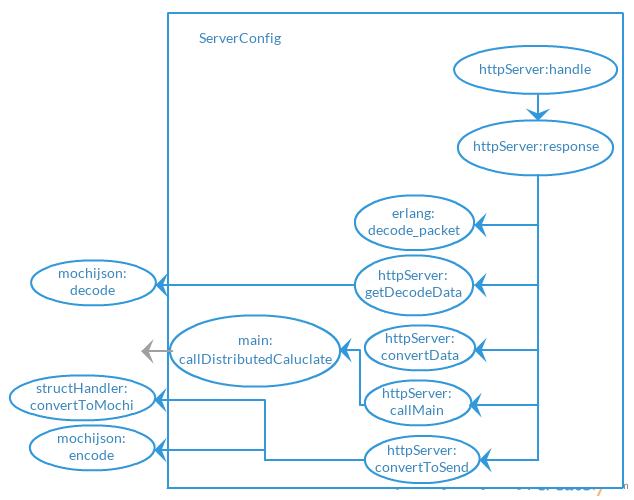
\includegraphics[width=13cm]{pics/call_graph_serverconfig}
		\centering
		\caption{Szerver hívási folyamata\label{fig:call_graph_serverconfig}}
	\end{figure}

	\begin{description}
	\item[httpServer:start(Port, WatcherNode)] 
		\hfill \\
		Elindítja a szervert, az adott porton. \newline
		Ezt a függvényt a main-ben hívjuk, meg ahol már megkapja a node-figyelő pid-jét és az alapértelmezett port-ot.
	\item[httpServer:response(Str, WatcherNode)] \hfill \\ 
		Miután érkezik egy kérés a szervernek ebben a függvényben kezeljük le. Innen indul ki minden folyamat ami a számítást végzi. \newline 
		Az alábbi sorrendben hívódnak meg a függvények: \newline
		getDecodeData, convertData, callMain, convertToSend.
	\item[httpServer:getDecodeData(\_)] \hfill \\ 
		Visszatér a szervernek küldött paraméterrel.
	\item[httpServer:convertData(ResponseParams)] \hfill \\ 
		Létrehozza a kapott adatból az Erlang struktúrát.
	\item[httpServer:callMain(RespJson, WatcherNode)] \hfill \\ 
		Amikor az adatokat feldolgoztuk és minden rendben ment, elindítjuk a main függvényét, ezen függvény segítségével.
	\item[httpServer:convertToSend(Object)] \hfill \\ 
		Amikor a számítás véget ért, létrehozzunk a visszaküldéshez szükséges adatstruktúrát, majd elküldjük a szervernek.
	\end{description}
\subsection{Adat feldolgozás}
	Az adatot JSON-ben kapja a szerver. Az adathalmaz kibontásához MonchiJSON lett alkalmazva. 
	A segédfüggvények és konvertálók a \texttt{Utility/structHandler.erl} fájlban lettek megvalósítva.\newline
	Elsősorban a megkapott speciális adathalmaz kibontására használtak az itt lévő függvények, de egyéb segédfüggvények is megtalálhatóak ebben a fájlban, amelyek a konvertálással kapcsolatosak.

	\subsubsection{\underline{
		Mochi-json kibontásához használt segédfüggvények:
	}}
	\begin{description}
		\item[structHandler:getElementByKeyList(KeyList, DataSetElement)] \hfill \\ 
		Visszatér egy értékkel, amely az adott kulcson van, ha egy elemű a kulcs lista. Több elem esetén a kulcsokban lévő értékeket nézi, és visszaadja a legbelső kulcson lévő elemet.

		\item[structHandler:getElementByKey()] \hfill \\ 
		Visszatér egy objektumban az adott kulcson lévő értékkel.
	\end{description}
	A struktúra-kezelő interpoláció meghívásához használt függvényei:
	\begin{description}

		\item[structHandler:getDataByJson(JsonSting)] \hfill \\
		A mochi-json dekódoló meghívása, visszatér egy Erlang struktúrával.
		
		\item[structHandler:getDataSet(Data)]\hfill \\ 
		Visszatér az adatok halmazával. Ebből a halmazon, vagyis listán kell végig menni, és szétosztani az elemeit. 
		
		\item[structHandler:getPoints] \hfill \\
		Pontok visszanyerése egy speciális módon, melyet a \texttt{calulator} fel tud használni.

				\begin{minted}{erlang}
EmptyStruct =  [{x, []}, {y, []}]
		\end{minted}


		\item[structHandler:<Számítási paraméterek>] \hfill \\ 
		getInverse(DataSetElement) - inverz-e \newline
		getType(DataSetElement) mi a típusa? \newline
		getId(DataSetElement) egyedi azonosítója \newline
		getPoints(DataSetElement) pontok struktúrája
	\end{description}
	Az eredmény visszanyeréséhez az alábbi segédfüggvényeket kellett használni:
	\begin{description}
	
		\item[structHandler:convertToMochi(Object)] \hfill \\ 
		A mochi-json Erlang struktúra annyira nem egyértelmű elemekből áll. Speciálisan kell felépíteni az eredményt. Ez a függvény megkap egy Erlang listát és átkonvertálja mochi-json-nak megfelelő struktúrává, majd átkonvertálja egy json string-gé.

		\item[structHandler:simplifyPolinomial(Result, Array) ] \hfill \\ 
		Egyszerűsíti a polinomot amelyet eredményül kapott.
	
	\end{description}
\subsection{Gép-szerver kommunikáció}
	\begin{description}
	\item[pidWatch:startPidWatch()]
	\hfill \\ Elindítja a node-figyelőt, melyben feliratkozni lehet a listára, vagy lekérdezni az adatokat. A node-figyelő indulás után figyelni fog és ha küldenek neki egy kérést, akkor azt kezeli. 
	\item[pidWatch:registerToServer(Pong\_Node)]
	\hfill \\ Ezzel a kéréssel lehet felcsatlakozni a szerverre. A kérést elküldi és ha sikeres volt a feliratkozás, akkor ok-al tér vissza.
	\end{description}
\subsection{Elosztás megvalósítása}
	Az elosztást tartalmazó fájlokat a /DistributedSystem mappában találjuk meg. nodeHandler.erl fájlban találhatóak a processz létrehozással kapcsolatos függvények. fork.erl fájlban a processz kommunikáció logikája van megvalósítva.

	%%\ref{fig:call_graph_distributed1}
	\begin{figure}[h]
		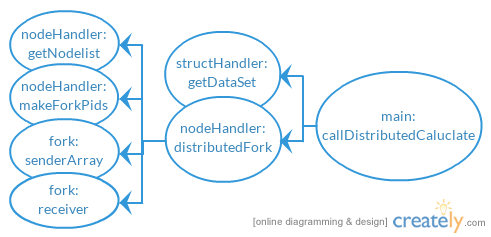
\includegraphics[width=10cm]{pics/call_graph_distributed1}
		\centering
		\caption{Elosztás folyamat hívásai\label{fig:call_graph_distributed1}}
	\end{figure}

	%%\ref{fig:call_graph_distributed1}
	\begin{figure}[h]
		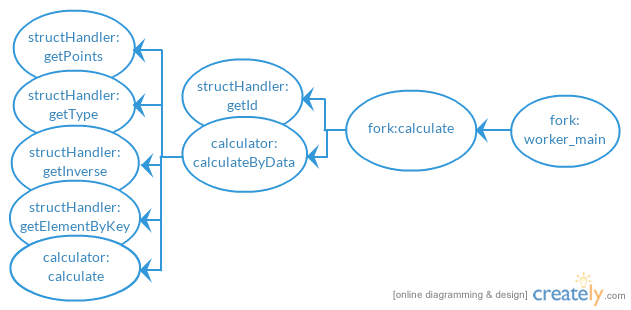
\includegraphics[width=12cm]{pics/call_graph_distributed2}
		\centering
		\caption{Gyerek folyamat hívásai\label{fig:call_graph_distributed2}}
	\end{figure}
	
	\begin{description}
		\item[nodeHandler:distributedFork(NumOfPids, DataList, WatcherNode)]
		\hfill \\
		Létrehozza a számításhoz szükséges node Struktúrát.
		LogicModule-ban szereplő senderstart, recivestart, worker\_main függvényeket kezeli.
		\item[nodeHandler:getNodelist]
		\hfill \\
		Lekéri a node-figyelőtől a felcsatlakozott node-okat.
		\item[nodeHandler:makeForkPids]
		\hfill \\
		Létrehozza a számításhoz szükséges új processzeket.

		\item[fork:senderArray]
		\hfill \\ 
			Végig megy egy adott tömbön és az elemeit szétküldi a processzeknek. 
		\item[fork:receiver]
		\hfill \\
			Válaszok érkezésére vár a processzektől. Ha minden válasz megérkezett, akkor visszatér.
		\item[fork:worker\_main]
		\hfill \\
			A gyerek processzek függvénye. Várja a szülőtől az adatot, számol vele és visszaküldi.
		\item[fork:calculate]
		\hfill \\ 
			A fork-ból a számítást hívó függvény. Eredménnyel visszatér, majd azt olyan formára hozza, amit vár a szülő. 
	\end{description}

%% ----------------------------------------------{Kalkulátor}
\section{Kalkulátor}
A Kalkulátor részben számítódik ki egy-egy interpolációnak az eredménye.
A megkapott adatok alapján számol, ha kell létre hozza a kezdő mátrixot, kiszámolja az eredmény mátrixot, majd annak segítségével kiszámolja a polinomot. \newline

\subsection{Felépítés}
	A számítást végző rész, nem áll sok fájlból, ezért ez nem lett sok részre szétbontva. 
	\begin{description}
		\item[calculator.cpp] 
		\hfill \\ Az egész számítás itt van megvalósítva, minden függvény, és segédfüggvény is.
		\item[erlang.cpp] 
		\hfill \\ Az Erlang-gal való kommunikáció megvalósítása
		\item[main.cpp] 
		\hfill \\ C++-os modul különálló tesztelésére kellett.
		\item[logTest.cpp] 
		\hfill \\ 
		Teszt függvények, melyekben dinamikus tesztesetek és paraméterezhető tesztesetek is vannak.
	\end{description}
\subsection{Fontosabb számítási függvények}
	\begin{description}
		\item[DArray interpolateMain] 
			\hfill \\ Kívülről meghívandó fő függvény mely elosztja és konvertálja a részeket
			\begin{description}
			  \item[DArray \&x :] Az x pontok listája 
			  \item[DMatrix \&Y :] Az x pontokhoz tartozó y pontok halmaza
			  \item[string type :] 
			  	Interpoláció típusa: Lagrange, Newton, Hermite
			  \item[bool inverse :] Inverz interpoláció kell-e
			\end{description}
		\item[void interpolateMatrix(DArray \&x, 	DMatrix \&M)] \hfill \\ 
			Interpolációs Táblázat kiszámítása
		\item[DArray l(int j, DArray X))] \hfill \\ 
			Lagrange polinom számítás segédfüggvénye
		\item[DArray getLagrangePolinomyal(DArray X, DArray Y)] \hfill \\ 
			Lagrange polinom számítás
		\item[DArray omega(int j, DArray X)] \hfill \\ 
			Newton polinom számítás segédfüggvénye
		\item[DArray polynomialAddition(DArray P, DArray Q)] \hfill \\ 
			polinom összeadás
		\item[DArray polynomialMultiply(DArray P, DArray Q)] \hfill \\ 
			polinom szorzás
		\item[DArray getPointsFromMatrix(DMatrix Y)] \hfill \\ 
			Pontokat(0. derivált) visszaadja a mátrixból
		\item[DMatrix getMatrixFromPoints(DArray Y)] \hfill \\ 
			Mátrixot ad vissza a pontokból
		\item[DArray getDiagFromMatrix (DMatrix \&M)] 
		\hfill \\
			Diagonális lekérése a mátrixból
		\item[void getInterpolationMatrix]
		\hfill \\  \textbf{(DArray X, DMatrix Y, DArray \&resX, DMatrix \&resM)}
		\hfill \\
			 X és Y ponthalmazból visszaadja a mátrixot 
	\end{description}
\subsection{Elosztott rendszerrel való kommunikáció}
	Az elosztott rendszerben hívódó számítást Erlang - erl\_nif"-el sikerült megoldanom. 
	Az ezzel kapcsolatos dolgokat az Calculator/erlang.cpp tartalmazza.
	\begin{description}
		\item[static ERL\_NIF\_TERM calculate\_nif] \hfill \\
		Ennek a függvénynek a segítségével valósul meg a kettő közötti kommunikáció
		\item[static int convertVector] \hfill \\
		Erlang lista C++ vektorrá konvertálása
		\item[static int convertMatrix] \hfill \\
		Erlang lista lista konvertálása C++ vektor vektorrá
		\item[static ERL\_NIF\_TERM convertList] \hfill \\
		Erlang listává konvertálás egy C++ vektorból
		\item[convertTheType] \hfill \\
			típus számot konvertálja string-gé: 
			"newton", "hermite", "lagrange"
		\item[static ErlNifFunc nif\_funcs] \hfill \\
			Felsorolja milyen függvényeket importálunk az Erlang-ba
	\end{description}
	Calculator/calculator.erl fájl tartalmazza az alábbi függvényeket: 
	\begin{description}
		\item[calculator:init()] \hfill \\
			"erlang:load\_nif" segítségével betölti a lefordított c++ fájlt.
		\item[calculator:calculate(\_X, \_Y, \_Type, \_Inverz)] \hfill \\
			Erre a függvényre lesz ráfordítva a C++-os függvény.
		\item[calculator:calculateByData(DataSetElement)] \hfill \\
		A bejövő paraméterből kinyeri a pontokat és a típust, majd meghívja a számító függvényt.
	\end{description}


\section{Tesztelési terv}
	A felület manuális teszteléssel lett kipróbálva, automatizált tesztesetek nem lesznek.
\subsection{Kalkulátor tesztelés}
	Ebben a részben a cpp-ben írt tesztesetekről lesz szó. \newline
	A tesztelést folyamatosan végeztem a minta adatok alapján. A függvények implementálása közben ezekre a minta adatokra meghívtam, majd ezekkel számoltam. A teszteléshez a logTest.cpp fájlban található függvényeket alkalmaztam. \newline
	A fájlban a javítást segítő kiírató függvények, integrációs teszt esetek, valamint manuális, felület nélküli számítást végző tesztesetek vannak. \newline
	Ezeket a teszteket nagyrészt kiváltották a szerveren futó tesztek, így fejlesztésük abba maradt, előfordulhat hogy a tesztek elavultak.
	\begin{description}
		\item[bool testAll()] \hfill \\ 
			Minden teszt lefuttatása. Ha minden teszt jól futott le akkor "true" értékkel tér vissza.
		\item[void testInterpolation(bool logPoly = false)] \hfill \\ 
			Interpolációs teszteket futtat.
			Mindegyik teszt egy egyszerű interpolációt vesz alapul, és a számítás eredményét ellenőrzi.
		\item[bool testMainInterpolation(bool logPoly = false)] \hfill \\ 
			Fő függvény tesztje. Elsősorban a feltétel átmeneteket teszteli, és azt hogy valóban számol-e ezen keresztül interpolációt.
		\item[bool testNewton(bool logPoly = false)] \hfill \\ 
			Newton számítás tesztje.
		\item[bool testLagrange(bool logPoly = false)] \hfill \\ 
			Lagrange interpoláció tesztje.
		\item[void testPolynomial()] \hfill \\ 
			Interpolációs mátrix tesztje.
		\item[void testMatrixInterpolation()] \hfill \\ 
			Manuális mátrix számítás függvénye.
		\item[void testManualInterpolation()] \hfill \\ 
			Manuális interpoláció számítás függvénye.

		\item[testManualPolynomial()] \hfill \\ 
			Manuális polinom összeadás és szorzás függvénye. 
		\item[void genXSquaredPoints(DArray \&X, DMatrix \&Y)] \hfill \\ 
			generál egy minta X,Y ponthalmazt az $x^{2}$ 
			pontjaiból.
		testMatrixInterpolation Segédfüggvénye
		feltölti az $x^{2}$ pontjaival.
	\end{description}
\subsection{Komponens és integrációs tesztelés}
	Főként az elosztást és a párhuzamosítást, valamint a szerveren lévő adatfeldolgozást teszteltem ilyen formában. Ezekkel a tesztesetekkel ellenőriztem a szerver és a számítás helyességét, és a szerver futást, miközben fejlesztettem.\newline
	Ezeket a teszteket érdemes lefuttatni, amikor a szervert konfiguráljuk. A szerveren lévő komponensek és azok egymással való kommunikációja fut le ilyenkor. Ha a teszten átmennek, akkor nagy valószínűséggel a szerveren már nem lehet probléma.\newline
	Viszont ha egy modul rosszul van leforgatva, vagy nincs betöltve, a tesztek hibát jeleznek. Ha a szerveren vagy gépen nem sikerült a tesztek lefutása, nem lehetséges a számítás elvégzése. Ennek oka valamelyik modul rosszul való betöltése, vagy az Erlang, GCC verziója nem megfelelő a számításokhoz.\newline
	Az átfogó tesztelés a ServerConfig/test.erl fájlban található. 
		\begin{description}
		\item[test:fork] \hfill \\
			Teszt futtatása a fork-nak ez a teszteset az párhuzamosítás miatt volt fontos. Viszont egy másik teszt átvette a helyét.
			\newline
			Ha mégis szükség lenne az általános párhuzamosítás tesztelésére, ezt kellene továbbfejleszteni.

		\item[test:runCheck, run] \hfill \\
			Futtatást kezelő függvények.
			Lefuttatják azokat a teszteket amiket a \\ 
			\texttt{ServerConfig/main.erl}-ből már el lehet indítani. 
			\newline \texttt{test:simulateDistributedCalculate} függvényt a main-ben található függvény tesztelésére használjuk, amit a bin/run.erl-ben lévő teszt futtat.
		\item[test:simulateDistributedCalculate] \hfill \\
			Egy olyan minta adatból, melyet a szerver is küldhet, elvégzi a számítást és ellenőrzi az eredményt. \newline
			Ha megadjuk neki a node-figyelő pid-jét akkor elosztott számítást is teszteli, és a node-figyelővel való kommunikációt. 
		\item[test:simplifyPolinomialTest] \hfill \\
			Ellenőrzi a struktúra kezelőben megvalósított polinom egyszerűsítést.  
		\item[test:convertMochiElements] \hfill \\
			structHandler: getTableData és getElementByKey tesztelésére írt függvény.
		\item[test:getResultTest] \hfill \\
			Eredmény konvertálásának tesztje. Szimulál egy processzektől visszakapható eredményt, majd ezt átalakítja a küldéshez megfelelő formátummá.
		\item[test:getParseJSONParams] \hfill \\
			Json string-ből a számításhoz szükséges minden paraméter kinyerésének tesztelése (structHandler teszt).
		\item[test:convertStruct] \hfill \\
			structHandler függvényeinek tesztje: \newline
			getNewPointStruct, appendNewPointStruct, convertPoints.
		\item[test:simulateFirstParseAndRun] \hfill \\
			Kibontja az első elemet a mintából, és számítás után ellenőrzi az eredmény helyességét. \newline
			Ez a teszt a számítást és az adat konvertálást teszteli, a párhuzamosítást/elosztást nem.
		\item[test:getFirstElementOfDataSet] \hfill \\
			Visszaadja a minta adatok első elemét.
		\item[test:getJSONString] \hfill \\
			Egy minta adathalmazt ad vissza (json string) ami jöhet a felületről.
		\item[test:getResultTestHelper] \hfill \\
			Számítási eredményekből és az elvárt eredményből a tesztelés eredményt állítja elő. 
	\end{description}

\subsection{Manuális tesztelés}
	Elsősorban a felület átfogó tesztelését végeztem ilyen módon, de a szerverrel való kommunikációnál és az elosztásnál is előkerültek ilyen módon hibák. \newline
	Az alábbi táblázatban felsoroltam a hibákat, melyek feltűntek a tesztelés során. 
	\begin{center}
  	\begin{tabular}{| p{4cm} | p{1.5cm} | p{8cm} |}
    \hline
    Hiba & Javítva & Info
  	\\ \hline
        Nem jó pontosság esetén nem jelenik meg a polinom
      &
      	igen
      &
		\textbf{Előidézés} : beírsz betűket a pontossághoz 
    \\ \hline
        Egy interpoláció adatbetöltési hibák
      &
      	igen
      &
      	Egy interpoláció tulajdonságainak betöltésénél nem állítja be az interpoláció típust és azt hogy inverz-e.
      	Nem jelenítjük meg a polinomokat sem bármilyen egyéb formában.
    \\ \hline
        Eredmény betöltésnél előfordul hogy a pontosság undefined 
      &
      	igen
      &
		\textbf{Előidézés?}:  Minta adatban fordul csak elő, de ha onnan  is betöltődhet akkor máshonnan is, amikor betölti az adatokat le kellene ezt kezelni.
   \\ \hline
    	Amikor pontot adunk hozzá nem frissül 
      &
      	igen
      &
		\textbf{Előidézés?}: Pont hozzáadása gomb esetén nem mentődnek el a háttérben az adatok
    \\ \hline
    	Hermite inverz nincs implementálva, és mégis beállítható a felületen.  
      &
      	igen
      &
		El tudjuk küldeni az oldalról úgy az adatokat hogy Hermite interpolációnál is állítható az inverz, közben a szerver nem inverz interpolációt fog számolni.
	\\ \hline
  \end{tabular}\end{center}
  \begin{center}\begin{tabular}{| p{4cm} | p{1.5cm} | p{8cm} |}
  \hline Hiba & Javítva & Info
    \\ \hline
      	Apache/2.2.22 verziónál a szerver nem működik. 
      &
      	igen
      &
		\texttt{[Sat May 09 17:20:18 2015] [crit] [client 192.168.1.153] configuration error:  couldn't perform authentication. AuthType not set!: /}\newline
		Server version: Apache/2.2.22 (Debian)
		Server built:   Jan 10 2015 15:33:51 
		\newline\textbf{Megoldás}:
		a régebbi verzió nem tudja kezelni a \texttt{"Require all granted"} kulcsszót.
	\\ \hline
        Node Lista lekérdezésnél valamikor végtelen ciklusba fut a lekérdezés. 
      &
      	igen
      &
      	\textbf{Hiba}:
		Hiba: túl sokszor küldjük el ugyanazt az üzenetet, és kapunk vissza rossz választ, kéne bele egy időkorlát is, a várakozásra. Másik hiba pedig hogy így egy régebbi üzenet lekezelése is megtörténhetett, így nem a legfrissebb node listát kaptuk meg. 
		\newline 
		\textbf{Megoldás}: Csak egyszer küldjük el, és ha rossz válasz érkezik, akkor tovább figyelünk.
  	\\ \hline
    	Szerver hiba bizonyos mennyiségű adatküldése felett 
      &
    	igen
      &  
    	\textbf{Előidézés}: 9-nél több egyszerű adat felküldése, minta nagy adatból 4db felett.
    	A szerver egybe küldi az értékeket, a httpServer modul már nem kapja meg a végét.
    	\textbf{Hiba}: A tcp kapcsolat nem záródik le, ezért bele kellett nyúlni az eredeti minta kód logikájába is.\newline
    	\textbf{Megoldás}: Bizonyos idő után lezárjuk a kapcsolatot Timeout-al, olyan idő lett megadva amelyben már remélhetőleg minden csomag megérkezik.
    \\ \hline
    	Erlang run:teszt és telepítés hiba a szerveren erlang 5.9.1 es verziónál
      &
      	nem
      &
      	\textbf{Telepítő futtatási hiba}: \newline
      	\texttt{escript: Internal error: badarg}
		\texttt{"init terminating in do\_boot"}
        \texttt{\{badarg,[\{io,format,[<0.29.0>,"~p",}
        \texttt{[[\{io\_lib,format ... }
		\newline \textbf{Teszt futtatásánál hiba}: \newline
		\texttt{exception error: no case clause matching <<127,248,0,0,0,0,0,0>>}
     	\texttt{in function  io\_lib\_format:mantissa\_exponent\/1}
     	\texttt{(io\_lib\_format.erl, line 374) }
    \\ \hline
	\end{tabular}\end{center}

  	\begin{center}\begin{tabular}{| p{4cm} | p{1.5cm} | p{8cm} |}
	\hline Hiba & Javítva & Info 
    \\ \hline
        Ha kilép egy node, akkor elszáll a számítás 
      &
      	nem
      &
      \textbf{Ötletek}:
      Node-ok kivételére is kellene opció,vagy kezelni kellene az elszálló node-okat.
      \newline Mielőtt elkezdjük a számítást, mindegyik node-ot ellenőrizzük, amelyik nem létezik már azt kivesszük a listából. Ha számítás közben hal meg: Bizonyos időközönként szintén küldünk egy ping-et az adott szervernek hogy létezik-e még. Ha meghalt a node akkor hibával tér vissza az adott számítás a kliensnek.
   	\\ \hline
    	Erlang: elosztási hiba
      &
      	nem
      &
      	Előfordul hogy a szerver elküldi a számító node-nak az adatot, az ki is számolja, viszont az eredmény nem érkezik vissza.\newline
      	A hiba elég véletlenszerűnek tűnik. Többször is elő tudtam igézni, majd amikor létrehoztam teljesen új elosztott rendszert egy vagy két gépen akkor már nem jelentkezett a hiba. 
    \\ \hline
  	\end{tabular}\end{center}

\newpage
\section{Összefoglaló}
	A kliens, mint weboldal egy komplex adathalmazt állít elő, nem csak a számítás, de a megjelenítés szempontjából is. Az adatok betöltődnek és elmentődnek, dinamikusan változnak az egyes pontokban. Rengeteg saját kézzel is szerkeszthető elemmel és táblázattal van tele a program. A grafikon kirajzolása mások által írt és ledokumentált program használata szintén egy érdekes és komplex feladat, kutatni kellett a megfelelő paraméterezéseket, és implementálni kellett egy segéd objektumot a használatára.\newline
	Emellett a szerver kommunikációt is meg kellett valósítani, mind a kliens, mind a szerver oldaláról. \newline
	Az Erlang dokumentációja és segédanyagai nem mindig voltak elegendőek, a hiba javítása igen nehézkes és lassú volt, viszont a párhuzamosítás megvalósítása után az elosztási rész egy szépen ledokumentált minta anyag segítségével könnyen használható volt. \newline  
	Az Erlang szerver kiépítése, és tesztelése még a szép minta programokkal sem volt annyira egyszerű, a problémái apache szerverrel lettek megoldva, amelynek konfigurálása még egy újabb feladat volt. \newline
	A számítás implementálása után, a szerverrel való össze kötése is egy kutató munka volt, és szerencsére az Erlang adott lehetőséget a C++-os modulok beépítésére, viszont ezzel is sok feladat adódott, mivel az adatokat át kellett konvertálni oda-vissza.
	\newline
	A probléma megoldásának egy igen komplex megvalósítása lett az eredmény, mely rengeteg kutatómunkát és fejlesztést tartalmaz.